\chapter{Acknowledgements}

\begin{center}
    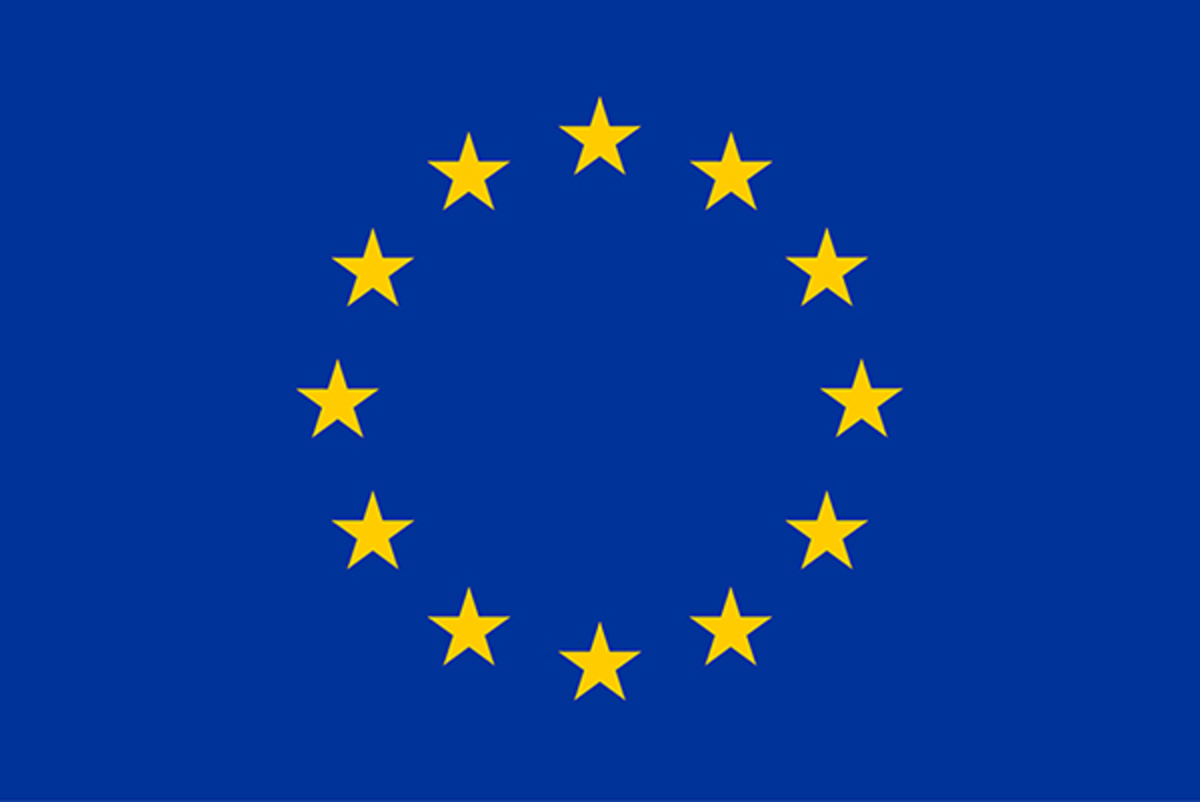
\includegraphics[width=0.25\textwidth]{0_Abstract/EU_Flag.pdf}
\end{center}

\noindent \textit{This Thesis is part of the "\acl{design}" project that has received funding from the \acl{eu}'s Horizon 2020 research and innovation programme under the Marie Skłodowska-Curie grant agreement No 860095.}

I thank the Cleanroom Operations Team of the \acl{brnc} for their help and support.
\vspace{\baselineskip}


\noindent This thesis is the culmination of a process that started around new year 2020, when I first found out the \acs{design} project was recruiting. My interest in semiconductors was first sparked during my master's degree at the Università degli Studi di Padova by the semiconductor physics course held by Prof. Davide de Salvador and Prof. Enrico Napolitani. A big thank-you goes to Prof. Raffaella Signorini, for her training and supervision during my master thesis, which introduced me to the world of III-V semiconductors and optoelectronics.

This project started in a particularly difficult year, in 2020, with the onset of COVID grinding all international travel to a halt. As an Italian citizen, my country was one of the first in Europe to be hit by the pandemic and by the time I was selected, it was not clear when exactly I would be able to enjoy the mobility required by this \acs{eu} project. I thank the team at IBM in Switzerland and the University of Glasgow for working hard to take advantage of the relaxation of quarantine measures that summer. 

I want to thank Prof. Kirsten Moselund for leading the MIND team that I was lucky to join, her ability in creating a strong team bond was conductive to a wonderful work environment. A big thank-you goes to Nele Harnack for all the sorties exploring Switzerland during the first year of our PhD. Another thank-you goes to Markus Scherrer and Preksha Tiwari for showing me the ropes of the \acs{tase} process and cleanroom etiquette, despite some questionable choices of wafer holder at the spin coater. The company of the MIND PhD students (and friends) was one of the personal highlights of my stay in Switzerland, whether at the lab or at the many outings in the alps, with a special mention to the Italy road trip.

I'm giving Ms. Marilyne Sousa her own paragraph as she stood out for her patience, kindness, trust, and attentive supervision during the entirety of my PhD. Marilyne always made me feel like I had an ally by my side, encouraging me in difficult moments and celebrating my achievements, no matter how little.

A special mention goes to the other \acs{esr}s in the \acs{design} project, Cristina Martinez Oliver and Christian Dam Vedel, for tolerating my breaking of the \acs{esr} naming convention with an "Enrico", patiently joining the (many) \acs{esr}-only meetings I organised, and overall being great to work with. A further acknowledgement goes to Cristina for her help during nanofabrication.

On the Glaswegian side, a thank-you goes to my academic supervisor Prof. Vihar Georgiev, who always led the \acs{design} project with a positive, can-do, attitude from the get go. This extends to the former Device Modelling and current Deep Nano members, in particular Preslav Alexantrov, for his irony coupled with long conversations on matters ranging from computer vision and machine learning to philosophy.

A mention goes to all the scientists, junior and senior, I met at conferences around the world for their friendliness and interesting insight.

Of course these four years weren't only filled with professional relationships, but with many personal ones too. I was fortunate enough to have many people share, if not all, at least pieces of this long, sometimes windy, road across Italy, Switzerland and Scotland, with me. Some of them were already mentioned, some other might not find a place here, but they all had a profound impact on my life, whether good or bad, in the last years. A huge thank-you goes to Audrey Liska, for her continued friendship and support, especially in times of hardship, and for the many adventures we shared meeting around Europe. Thank you to the old friends from Italy, Martina Marasi, Nico Ragazzo, and Gabriele Baldon, shared a bit of my adventure in Switzerland, and Lorenzo Cazzola and Daniele Chilò were always available for a spritz, a card game, and many laughs when I was back in Italy. A mention goes out to the "Fioi" group, which, while more and more scattered around Europe, still had great stories during our meetups. Another special mention goes out to the Scottish components of the "Mumble" group, for their linguistic and cultural tutoring, as well as the endless and (mostly) tasteful banter.

Last but by far not least, a big thank you to my family, starting with my parents Pietro and Annamaria, without whom I quite literally would not be here, and my sister, Isabella, and extending to my aunts, uncles, and cousins, for always supporting me during my "thesis on light bulbs". A final thought goes out to my grandparents, who are not here anymore, but to whom I always look back in these moments, for teaching child me many of the values I hold dear in life to this day.